% \documentclass[mat1, tisk]{fmfdelo}
\documentclass[mat1]{fmfdelo}
\usepackage{graphicx}
\usepackage{float}

\avtor{Gregor Kikelj}
\naslov{Preverjanje kromatičnega števila grafov z dokazovalnim pomočnikom Lean}
\title{Verification of chromatic number of a graph with Lean proof assistant}
\mentor{prof. dr. Andrej Bauer}
\letnica{2024}

% - povzetek v slovenščini
%   V povzetku na kratko opišite vsebinske rezultate dela. Sem ne sodi razlaga
%   organizacije dela, torej v katerem razdelku je kaj, pač pa le opis vsebine.
\povzetek{TODO}

% - povzetek v angleščini
\abstract{TODO}

% - klasifikacijske oznake, ločene z vejicami https://www.ams.org/msc/
\klasifikacija{68R10}
\kljucnebesede{...\sep ...}
\keywords{...\sep ...}

\slovar{
\geslo{Chromatic number}{Kromatično število}
}

% - ime datoteke z viri (vključno s končnico .bib), če uporabljate BibTeX
% \literatura{....bib}
\usepackage{hyperref}
\usepackage{listings}
\usepackage{color}
\definecolor{keywordcolor}{rgb}{0.7, 0.1, 0.1}   % red
\definecolor{tacticcolor}{rgb}{0.0, 0.1, 0.6}    % blue
\definecolor{commentcolor}{rgb}{0.4, 0.4, 0.4}   % grey
\definecolor{symbolcolor}{rgb}{0.0, 0.1, 0.6}    % blue
\definecolor{sortcolor}{rgb}{0.1, 0.5, 0.1}      % green
\definecolor{attributecolor}{rgb}{0.7, 0.1, 0.1} % red

\def\lstlanguagefiles{lstlean.tex}
\lstset{language=lean}
\usepackage{titlesec} 
\titleformat{\section}[block]
  {\normalfont\Large\bfseries}{\thesection}{1em}{}
\titlespacing*{\section}{1mm}{\baselineskip}{\baselineskip}



\begin{document}
\section{Uvod}
Raziskovanje kromatičnega števila grafov predstavlja pomemben problem teorije grafov.
Kromatično število grafa nam pove najmnaj koliko barv potrebujemo za barvanje vozlišč grafa, tako da dve sosednji vozlišči nista enake barve.
Ta problem ni zanimiv le matematično, ampak ima uporabe tudi pri drugih področjih, predvsem v povezavi z računalništvom. 
Iskanje kromatičnega števila je sicer računsko težek problem v smislu, da ne poznamo algoritma, ki bi ga računal v polinomskem času v odvisnosti od števila vozlišč grafa.

V tej diplomski nalogi se osredotočimo na iskanje kromatičnega šteila skupaj z dokazom da smo res našli pravo vrednost.
Da to dosežemo si bomo pomagali z dokazovalnikom Lean.
V prvem delu naloge natančno definiramo pojme iz teorije grafov ki jih potrebujemo za dokazovanje. Nato na kratko opišemo osnove uporabe dokazovalnika
Lean ter matematične definicije konstruiramo znotraj Leana. 
Na koncu definiramo nekaj algoritmov za iskanje kromatičnega števila in dokažemo njihovo pravilnost. 


\section{Osnove teorije grafov in kromatično število}

\begin{definicija}
    Graf je urejen par $G=(V, E)$ kjer je 
    \begin{itemize}
      \item $V\neq \emptyset$ končna množica vozlišč,
      \item $E$ množica povezav, kjer je vsaka povezava množica dveh različnih vozlišč iz $V$. 
    \end{itemize}
\end{definicija}
Če sta različni vozlišči $u, v$ elementa neke povezave iz $E$ to pišemo kot $u\sim v$ ter pravimo, da sta sosednji vozlišči in da sta krajišči povezave $uv\in E$.

\begin{figure}[H]
\begin{center}
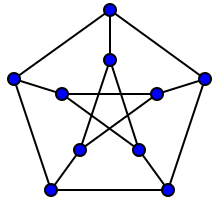
\includegraphics[scale=1]{assets/graph}
\caption{Primer grafa}
\label{slika2}
\end{center}
\end{figure}

\begin{definicija}
    Naj bo $v\in V$. Stopnja vozlišča $v$ je število elementov $E$ ki vsebujejo $v$, oziroma z besedami število povezav, ki vsebujejo $v$. 
\end{definicija}

\begin{itemize}
    \item Največjo stopnjo v grafu označimo z \[\Delta (G) = \max_{v\in V} deg(v)\]
    \item Najmanjšo stopnjo v grafu označimo z \[\delta (G) = \min_{v\in V} deg(v)\]
\end{itemize}

\begin{definicija}
    Definiramo oznako $[k] = \{0, 1, 2, \dots, k-1\}$ za množico naravnih števil manjših od $k$.
\end{definicija}

\begin{definicija}
    Naj bo $G$ graf in $k\in \mathbb{N}$. Preslikava $f:V(G)\to [k]$ je $k$ barvanje grafa $G$ če za vse $u, v\in V$ velja $u\sim v \implies f(u)\neq f(v)$.
\end{definicija}
Z besedami: barvanje grafa s $k$ barvami je preslikava, ki vsakemu vozlišču priredi eno izmed $k$ barv, tako da sta sosednji vozlišči vedno pobarvani z različnima barvama.
\begin{figure}[H]
    \begin{center}
    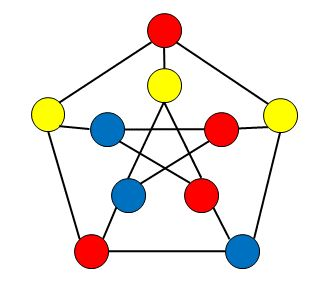
\includegraphics[scale=0.5]{assets/coloring}
    \caption{Primer barvanja grafa}
    \label{slika2}
    \end{center}
    \end{figure}
    
\begin{definicija}
    Kromatično število grafa $G$ ki ga označimo kot $\chi(G)$, je najmanjše število, da obstaja $\chi(G)$ barvanje grafa $G$.
\end{definicija} 
\begin{lema}
    Naj bo $G$ graf. Potem kromatično število grafa $G$ obstaja.
\end{lema}
\begin{dokaz}
    Dovolj je da dokažemo da obstaja neko število $k$ za katerega obstaja $k$ barvanje grafa $G$.
    Dokažimo da je $k=|V|$ dovolj, kjer je $V$ množica vozlišč grafa $G$. Ker je $V$ končna množica
    lahko vozlišča oštevilčimo kot $V = \{v_0, v_1, \dots, v_{k-1}\}$. Poglejmo si barvanje 
    \[ f:V \to [k], f(v_i) = i\]
    Dokazati moramo $\forall v_i, v_j \in V, v_i \sim v_j\implies f(v_i)\neq f(v_j)$. Po definiciji $f$ je dovolj dokazati
    $\forall v_i, v_j \in V, v_i \sim v_j\implies i\neq j$. Obrnemo implikacijo in dokazujemo $\forall v_i, v_j \in V, i=j \implies
    v_i \nsim v_j$. To sledi iz definicije množice povezav grafa kjer je povezava množica dveh različnih vozlišč. 
\end{dokaz}

\begin{definicija}
Naj bosta $G$ in $H$ grafa. Pravimo da je $H$ podgraf $G$ če je $V(H)\subset V(G)$ in $E(H)\subset E(G)$.
\end{definicija}
\begin{lema}
    Naj bo $G$ graf in $H$ njegov podgraf. Naj bo $f$ barvanje grafa $G$. Potem je omejitev barvanja $f$ na vozlišča
    grafa $H$ veljavno barvanje grafa $H$.
\end{lema}
\begin{proof}
Naj bo $f:V(G)\to [k]$ barvanje grafa $G$. Dokažimo da je omejitev barvanja $f$ na vozlišča grafa $H$ veljavno barvanje grafa $H$.
Dovolj je dokazati $\forall v_i, v_j \in V(H), v_i \sim v_j\implies f(v_i)\neq f(v_j)$. Naj bosta torej $v_i, v_j \in V(H)$, 
da velja $v_i \sim v_j$. Ker je $H$ podgraf $G$ velja tudi $v_i, v_j \in V(G)$ ter $v_i \sim v_j$ v $G$. Ker je $f$ veljavno barvanje
grafa $G$ je $f(v_i)\neq f(v_j)$.
\end{proof}


\begin{lema}
    Naj bo $G$ graf in $H$ njegov podgraf. Potem velja $\chi(H)\leq \chi(G)$.
\end{lema}
\begin{proof}
    Naj bosta $C_G$ in $C_H$ množici kjer je $k\in C_G$ čee obstaja $k$ barvanje grafa $G$. Potem je kromatično število
    grafa $G$ enako najmanšemu elementu $C_G$. Dovolj je dokazati da je $C_H\subset C_G$, ker je minimum podmnožice vedno
    manjši ali enak minimumu celotne množice. Ker je $H$ podgraf $G$ je vsako barvanje grafa $G$ tudi barvanje grafa $H$.
    Torej, če obstaja $k$ barvanje grafa $G$ obstaja tudi $k$ barvanje grafa $H$, zato je $C_H\subset C_G$.
\end{proof}


\section{Dokazovalni pomočnik Lean}
Lean je interaktivni dokazovalni pomočnik. Uporabljali bomo verzijo Lean 4 ki je razvita pri Microsoftu in temelji na teoriji tipov
s čimer se ne bomo ukvarjali preveč ker je tema te diplomske naloge teorija grafov. Lean 4 bomo uporabljali tudi
kot funkcijski programski jezik. Za bolj natančne podrobnosti o Leanu priporočamo ogled uradne dokumentacije. 

\subsection{Računanje izrazov}
Kot ostali običajni programski jeziki tudi Lean podpira računanje osnovnih aritmetičnih izrazov.
\begin{lstlisting}
#eval 1 + 1
\end{lstlisting}
Lean nam v informacijskem oknu pove da se izraz evaluira v 2. Lean upošteva tudi vrstni red operacij na primer
\begin{lstlisting}
#eval 1 + 2 * 3
\end{lstlisting}
se izračuna v 7. Če želimo uporabiti drugačen vrstni red operacij lahko to naredimo z oklepaji
\begin{lstlisting}
#eval (1 + 2) * 3
\end{lstlisting}
ki se izračuna v 9.


\subsection{Tipi}
Tipe poznamo iz drugih programskih jezikov (npr. Python, Java) so pa v Leanu bolj pomembni in imajo nekaj več funkcionalnosti.

Osnovni tipi s katerimi se bomo največ ukvarjali so:
\begin{itemize}
    \item \lstinline{Nat} naravna števila
    \item \lstinline{Int} cela števila
    \item \lstinline{String} nizi
    \item \lstinline{List} seznami
\end{itemize}
Lean načeloma tipe izrazov ugotovi sam, lahko pa jih tudi podamo. Na primer
\begin{lstlisting}
#eval 2
\end{lstlisting}
se izračuna v 2, Lean pa nam pove da je tip izraza \lstinline{Nat}. Če pa želimo izraz izračunati kot \lstinline{Int} lahko to naredimo z
\begin{lstlisting}
#eval (2 : Int)
\end{lstlisting}
kar nam potem predstavlja 2 kot celo število. Lean ponavadi namesto
\lstinline{Nat} uporabi oznako \lstinline{ℕ} in namesto \lstinline{Int} oznako \lstinline{ℤ}, to pa lahko uporabljamo tudi mi
da se program bolj ujema z matematičnim zapisom. 

Poglejmo si sedaj kako definiramo funkcije
\begin{lstlisting}
def f (x : ℕ) : ℕ := x + 1
\end{lstlisting}
Definirali smo funkcijo \lstinline{f} ki sprejme naravno število in vrne naravno število. Funkcijo lahko poračunamo podobno kot izraze
\begin{lstlisting}
#eval f 2
\end{lstlisting}
ki se izračuna v 3. Če nismo prepričani kakšen tip ima nek objekt v leanu lahko to ugotovimo z ukazom
\begin{lstlisting}
#check f
\end{lstlisting}
ki nam vrne \lstinline{ℕ → ℕ} torej je funkcija $f$ preslikava iz naravnih števil v naravna števila.

Lahko definiramo tudi funkcije več spremenljivk
\begin{lstlisting}
def vsota (x: ℕ) (y: ℕ) : ℕ := x + y
\end{lstlisting}
ki ima tip \lstinline{ℕ → ℕ → ℕ} torej je preslikava iz naravnih števil v preslikave iz naravnih števil v naravna števila.
Ker imata oba argumenta funkcije isti tip lahko definicijo skrajšamo
\begin{lstlisting}
def vsota (x y: ℕ) : ℕ := x + y
\end{lstlisting}
Ker lean zna sam ugotoviti tip vsote dveh naravnih števil tega ni potrebno podati je pa včasih to bolj berljivo
\begin{lstlisting}
def vsota (x y: ℕ) := x + y
\end{lstlisting}
Še krajše pa gre z lambda zapisom in spuščanjem nekoristnih presledkov.
\begin{lstlisting}
λx y:ℕ=>x+y
\end{lstlisting}

Lean v funkcijah podpira tudi bolj "običajno" programiranje. Lahko recimo definiramo pomožne spremenljivke
\begin{lstlisting}
def funkcija (a:Nat) : Nat := 
  let b := a+1
  b*b
\end{lstlisting}

Lahko tudi kličemo druge funkcije
\begin{lstlisting}
def funkcija2 (a:Nat) : Nat :=
    let b := funkcija a
    b*b
\end{lstlisting}

Imamo tudi možnost uporabe stavka \lstinline{if}
\begin{lstlisting}
def funkcija3 (a:Nat) : Bool :=
  if a = 0 then
    true
  else
    false
\end{lstlisting}
Uporabljamo lahko tudi rekurzijo.
\begin{lstlisting}
def funkcija4 (a:Nat) : Nat :=
    if a = 0 then
      0
    else
      1 + funkcija4 (a-1)
\end{lstlisting}
kjer pa moramo poskrbeti da se rekurzija zaključi. Včasih Lean pri tem potrebuje nekaj pomoči, detajli o tem so izven obsega te diplomske naloge.

Seveda lahko staveke if, rekurzijo in pomožne spremenljivke uporabljamo tudi v funkcijah več spremenljivk.
\begin{lstlisting}
def vecje (n : Nat) (k : Nat) : Nat :=
  if n < k then
    k
  else n
\end{lstlisting}
Ker ima funkcija \lstinline{vecje} dva argumenta je tip \lstinline{ℕ → ℕ → ℕ}. Kot v OCamlu lahko tudi tukaj funkciji podamo en argument 
da dobimo fukncijo tipa \lstinline{ℕ → ℕ}.
\begin{lstlisting}
def dodaj5 := vsota 5
\end{lstlisting}

Na primer \lstinline{dodaj5 3} se izračuna v 8.


\subsection{Podatkovne strukture}

Podobno kot v večini programskih jezikov obstajajo razredi, lahko tudi v Leanu definiramo strukture, ki so ponavadi namenjene temu da združimo več podatkov v en objekt.
\begin{lstlisting}
structure Tocka :=
    x: Nat
    y: Nat
\end{lstlisting}
Objekt neke strukture definiramo tako da navedemo vrednosti vseh polj
\begin{lstlisting}
def izhodisce : Tocka := {x := 0, y := 0}
\end{lstlisting}
Tudi te tipe lahko uporabljamo kot argumente ali rezultate funkcij.
Dostop do posameznih komponent strukture je podoben kot v večini programskih jezikov
\begin{lstlisting}
#eval izhodisce.x
\end{lstlisting}
torej z \lstinline{ime_objekta.ime_komponente}.

\subsubsection{Induktivni tipi}
Poleg struktur ki zapakirajo več podatkov v en objekt, Lean podpira tudi induktivne tipe, ki nam omogočajo, da definiramo objekt nekega tipa
kot eno izmed končne množice možnosti. Na primer tip \lstinline{Bool} je induktivni tip, ki ima dve možnosti \lstinline{true} in \lstinline{false}.
\begin{lstlisting}
inductive Bool where
| false : Bool
| true : Bool
\end{lstlisting}

Bolj realen primer bi bil recimo dan v tednu
\begin{lstlisting}
inductive DanVTednu where
| ponedeljek : DanVTednu
| torek : DanVTednu
| sreda : DanVTednu
| cetrtek : DanVTednu
| petek : DanVTednu
| sobota : DanVTednu
| nedelja : DanVTednu
\end{lstlisting}

Induktivni tipi podpirajo \lstinline{match} stavke, ki so nekoliko podobni \lstinline{switch} stavkom v drugih programskih jezikih.

\begin{lstlisting}
def negacija (b:Bool) : Bool :=
  match b with
  | true => false
  | false => true
\end{lstlisting}

\begin{lstlisting}
def jeVikend (d:DanVTednu) : Bool :=
    match d with
    | DanVTednu.sobota => true
    | DanVTednu.nedelja => true
    | _ => false
\end{lstlisting}

Vidimo da lahko podobno kot v OCamlu uporabljamo tudi \lstinline{_} kot "wildcard" v match stavku.
Objekti induktivnega tipa so lahko definirani tudi rekuzivno.
\begin{lstlisting}
inductive Nat where
    | zero : Nat
    | succ (n : Nat) : Nat
\end{lstlisting}
Torej naravno število je lahko 0 ali pa naslednik naravnega števila. Tudi pri taki definiciji lahko uporabljamo \lstinline{match} stavke
in vsa ostala orodja ki jih Lean ponuja.

Pomemben induktivni tip je tudi \lstinline{List} ki predstavlja sezname in je primer parametričnega tipa.
\begin{lstlisting}
inductive List (α : Type) where
    | nil : List α
    | cons : α → List α → List α
\end{lstlisting}


\section{Formalizacija in računanje kromatičnega števila}
\subsection{Formalizacija kromatičnega števila}
Pogjemo si definicijo kromatičnega števila v Leanu.
Za berljivost bomo večino dokazov spuščali.
Celotna koda je dostopna na \url{https://github.com/grekiki2/Lean-tests}.
Vsekakor je v primerjavi s papirjem, boljše dokaze pregledovati znotraj urejevalnika npr. VSCode, ki nam omogoča da v vsakem delu dokaza vidimo 
trenutne predpostavke in željen rezultat. 

\begin{lstlisting}
structure Graph :=
    vertexSize : Nat
    connected: Fin vertexSize → Fin vertexSize → Pro
    connected_decidable: ∀ a b, Decidable (connected a b)
    irreflexive: ∀ n, ¬ connected n n
    symmetric: ∀ a b, connected a b → connected b a
\end{lstlisting}
Graf torej definiramo kot strukturo kjer podamo število vozlišč, izračunljivo funkcijo ki nam pove
ali sta dve vozlišči povezani ter potrdilo da je relacija povezanosti irefleksivna in simetrična.

Za namene testiranja definiramo še graf $K_n$, ki je graf z $n$ vozlišči in povezavami med vsemi pari vozlišč.
\begin{lstlisting}
def K_n (k:Nat): Graph :=
  {vertexSize:=k, connected:=(λ x y=>x ≠ y), connected_decidable := by simp; intro a b;apply Not.decidable, irreflexive := by simp, symmetric:= by apply Ne.symm }
\end{lstlisting}
Na podoben način definiramo tudi $C_n$ oziroma cikličen graf z $n$ vozlišči le da moramo podati še dokaz da je $n\ge2$.

Definicija grafa ki smo jo naredili je precej splošna in jo lahko uporabimo tudi za definicje grafov iz seznama povezav.
Recimo da imamo spremenljivko \lstinline{edges :  Array (Array (Fin n)) } ki predstavlja seznam sosednosti grafa.
Potem lahko definiramo splošen graf kot
\begin{lstlisting}
let g1 : Graph := {
    vertexSize := n
    , connected := λ x y => x≠y ∧ (y ∈ edges[x]'(by rw [h]; exact Fin.prop x) ∨ x ∈ edges[y]'(by rw [h]; exact Fin.prop y))
    , connected_decidable := by {
        intro x y
        simp
        apply And.decidable
    }
    , irreflexive := by {
        intro a
        simp
    }
    , symmetric := by {
        intro a b
        simp
        intro h h2
        constructor
        · exact Ne.symm h
        · exact Or.symm h2
    }
}
\end{lstlisting}
Podobno bi lahko naredili tudi z grafom ki bi za seznam sosednjosti uporabljal tip \lstinline{List}, vendar pa je uporaba \lstinline{Array} 
bolj učinkovita.

Definiramo še tip ki predstavlja $k$ barvanje grafa
\begin{lstlisting}
def Coloring (G:Graph) (k : Nat) := Fin G.vertexSize → Fin k
\end{lstlisting}

Predstavili smo $k$ barvanje grafa kot preslikavo iz (indeksa) vozlišča v eno izmed $k$ barv.
Definiramo še kdaj je $k$ barvanje veljavno
\begin{lstlisting}
def valid_coloring (G:Graph) {k:Nat} (coloring: Coloring G k): Prop :=
  ∀ a b, GraphConnected G a b → coloring a ≠ coloring b
\end{lstlisting}
Sledimo definiciji iz drugega poglavja. Torej z besedami, barvanje je veljavno 
če sta sosednji vozlišči vedno pobarvani z različnima barvama.

Ker preslikava preverja povezanost za končno število elementov se lahko uporablja za računanje. Drugače rečeno, smiselno
je napisati
\begin{lstlisting}
#eval valid_coloring (K_n 5) (λ x => 0)
\end{lstlisting}
in pričakovati da Lean to izračuna. Lean na žalost izračunljivosti tega izraza ne ugotovi sam, zato moramo pokazati, 
da je \lstinline{valid_coloring} izračunjiv oz v Leanu decidable.
\begin{lstlisting}
instance (G: Graph) (k:Nat) (coloring: Coloring G k): Decidable (@valid_coloring G k coloring)
    exact Nat.decidableForallFin _
\end{lstlisting}

Zdaj lahko torej za neko barvanje z Leanom preverimo ali je veljavno ali ne. 
Ker je množica barvanj grafa $G$ s $k$ barvami končna lahko definiramo tudi izračunljivo funkcijo ki nam 
za graf $G$ pove ali obstaja $k$ barvanje
\begin{lstlisting}
def is_k_colorable (G : Graph) (k: Nat) : Prop :=
  ∃ (coloring : Coloring G k), valid_coloring G coloring
\end{lstlisting}

Tudi ta funkcija je izračunljiva ker je množica barvanj grafa $G$ s $k$ barvami končna.
\begin{lstlisting}
instance {G : Graph} (k : Nat) : Decidable (is_k_colorable G k) := Fintype.decidableExistsFintype
\end{lstlisting}

Sedaj lahko končno definiramo kromatično število grafa $G$ kot najmanjše število $k$, da velja
\lstinline{is_k_colorable G k}. V Leanu(oziroma bolj natančno Mathlibu) to naredimo s pomočjo funkcije \lstinline{Nat.find}
ki kot argumente vzame:
\begin{itemize}
    \item \lstinline{p : Nat → Prop} Izračunljiv predikat za katerega iščemo najmanjše število da velja \lstinline{p}
    \item \lstinline{h : ∃ n, p n} dokaz da obstaja neko naravno število za katerega velja \lstinline{p}
\end{itemize}

Definicija kromatičnega števila v Leanu je potem
\begin{lstlisting}
def ChromaticNumber (G: Graph): ℕ :=
  @Nat.find (is_k_colorable G) _ (by {
    unfold is_k_colorable valid_coloring GraphConnected
    use G.vertexSize, λ i=>i
    intro a b hab
    by_contra h
    simp [← h] at hab
    exact (G.irreflexive a) hab
  })
\end{lstlisting}
Vzamemo torej najmanjše število barv da je graf $G$ $k$ barvljiv, zraven pa dokažemo da vsaj eno tako število obstaja.
Najbolj preprosto to naredimo tako da vzamemo število vozlišč grafa $G$ in definiramo barvanje ki vsakemu vozlišču priredi njegov indeks.
V poglavju 2 smo se prepričali, da je to res veljavno barvanje.

\subsection{Računanje kromatičnega števila}
Funkcijo \lstinline{chromatic_number} lean prepozna kot izračunljivo in jo lahko že uporabljamo za interaktivno računanje
kromatičnega števila. Na primer
\begin{lstlisting}
#eval ChromaticNumber (K_n 8)
\end{lstlisting}
nam vrne 8 (po nekaj sekundah). Podobno nam
\begin{lstlisting}
#eval ChromaticNumber (C_n 13 (by linarith))
\end{lstlisting}
vrne 3 in
\begin{lstlisting}
#eval ChromaticNumber (C_n 14 (by linarith))
\end{lstlisting}
vrne 2. Za računanje kromatičnega števila seveda obstajo hitrejši algoritmi kot je naš, 
ki to dela na način da preveri vsa možna barvanja pri nekem $k$ dokler ne najde veljavnega, ali pa gre 
na naslednji $k$, vendar pa je dokazovanje pravilnosti kompleksnejših algoritmov izredno kompleksno.

Lahko pa si pomagamo s t.i.\ pričami. Vemo, da če imamo neko barvanje grafa s tremi barvami, je kromatično število največ 3. 
Barvanje lahko poišče nek kompleksen algoritem, Lean pa mora potem le preveriti da je veljavno. Da si bomo lahko pomagali s takimi
prijemi, pa potrebujemo nekaj pomožnih lem. 

Najprej bomo pokazali da če obstaja $k$ barvanje grafa $G$, je kromatično število grafa $G$ največ $k$. Da to storimo pa potrebujemo
lemo ki nam pove da iz barvanja grafa $G$ s $k$ barvami lahko tvorimo barvanje grafa $G$ z $l$ barvami, če je le $l\geq k$.
\begin{lstlisting}
def extend_coloring (G:Graph) (k1 k2: Nat) (h:k2≥k1) (coloring: Coloring G k1) (h2: valid_coloring G coloring):∃ coloring2:Coloring G k2, valid_coloring G coloring2
\end{lstlisting}
Nato lahko dokažemo da $k$ barvanje grafa $G$ obstaja če in samo če je kromatično število grafa $G$ največ $k$.
\begin{lstlisting}
lemma colorable_gives_ub (G: Graph) (k: Nat):
    is_k_colorable G k ↔ chromatic_number G ≤ k
\end{lstlisting}
\begin{proof}
Najprej dokažimo implikacijo v desno. Kromatično število smo definirali kot najmanjši $i$ da je graf $G$ $i$ barvljiv.
Če je torej graf $G$ $k$ barvljiv potem je kromatično število grafa $G$ največ $k$.
V levo, če vemo da je kromatično število grafa $G$ največ $k$ potem obstaja barvanje grafa $G$ z največ $k$ barvami
ki ga lahko razširimo do barvanja s $k$ barvami po lemi \lstinline{extend_coloring}.
\end{proof}

Posledica je da če in samo če barvanje s $k$ barvami ne obstaja je $k$ manjši od kromatičnega števila grafa $G$.
\begin{lstlisting}
lemma not_colorable_gives_lb (G: Graph) (k: Nat) :
    ¬ is_k_colorable G k ↔ k < chromatic_number G
\end{lstlisting}

Iz navedenega dobimo glavno posledico.
Če najdemo nek $k$ da graf $G$ ni $k$ barvljiv je pa $k+1$ barvljiv potem je kromatično število grafa $G$ enako $k+1$.
\begin{lstlisting}
theorem bounds_give_chromatic (G:Graph) (k: Nat):
    ¬is_k_colorable G k ∧ is_k_colorable G (k+1) ↔ chromatic_number G = k+1
\end{lstlisting}

Če sedaj na dokazano gledamo iz vidika uporabnosti je precej preprosto Leanu razložiti da je graf $G$ $k$ barvljiv
(če je to res, razlaganje napačnih stvari načeloma naj ne bi bilo mogoče) recimo tako da najdemo neko barvanje. Večji problem pa je
s spodnjo mejo kromatičnega števila. 
V tem delu se bomo spodnje meje lotili s pomočjo podgrafov.


\subsection{Podgrafi}
Dokažimo naslednji izrek
\begin{lstlisting}
theorem subgraph_chromatic_number_le (G G2:Graph) (f:Fin G2.vertexSize → Fin G.vertexSize) (f_inherits: ∀ a b, G2.connected a b → G.connected (f a) (f b)):
    ChromaticNumber G2 ≤ ChromaticNumber G
\end{lstlisting}
Uporabili smo definicijo podgrafa ki je bolj primerna za Lean kot standardna definicija.
Graf $G2$ je podgraf grafa $G$ če obstaja preslikava $f$ ki vozlišča $G2$ preslika v vozlišča $G$ tako, 
da če sta vozlišči v $G2$ povezani sta povezani tudi preslikani verziji teh vozlišč v $G$.

Izrek pravi da če je $G'$ podgraf $G$, potem je kromatično število grafa $G'$ manjše ali enako kromatičnemu številu grafa $G$.
\begin{proof}
Po definiciji kromatičnega števila je dovolj dokazati, da lahko graf $G'$ pobarvamo z $\chi(G)$ barvami. Naj bo $c_G$ 
neko $\chi(G)$ barvanje grafa $G$. Trdimo da je $c_{G'}$ definirano kot $c_{G'}(i) = c_G(f(i))$ veljavno barvanje grafa $G'$. 
Barvanje je veljavno če sta sosednji vozlišči vedno pobarvani z različnima barvama. Naj bosta $a, b$ sosednji vozlišči grafa $G'$.
Potem sta po definiciji podgrafa sosednji tudi vozlišči $f(a), f(b)$ v grafu $G$. Ker je $c_G$ veljavno barvanje grafa $G$, je 
$c_G(f(a))\neq c_G(f(b))$. Ker je $c_{G'}(a) = c_G(f(a))$ in $c_{G'}(b) = c_G(f(b))$ je tudi $c_{G'}(a)\neq c_{G'}(b)$.
\end{proof}
Opomba: pri definiciji podgrafa bi načeloma morali zahtevati injektivnost vendar pa je nikjer v dokazih ne potrebujemo zato
tega v Leanu nismo naredili. 

Zdaj si lahko pomagamo pri iskanju spodnjih mej kromatičnega števila tako da najdemo nek manjši podgraf ki 
ima čim večje kromatično število. V praksi se recimo pogosto uporablja $K_n$ klike ki imajo kromatično število $n$, 
ali pa $C_n$ ciklični grafi ki imajo kromatično število $2$ če je $n$ sodo in $3$ če je $n$ liho število.

V delu se bomo osredotočili na ciklične grafe.

\subsection{Kromatično število cikličnih grafov}
Dokažimo da je kromatično število cikličnega grafa s sodim številom vozlišč enako $2$.
\begin{lstlisting}
theorem chromatic_number_of_C_n_even (n:Nat) (h:2*n≥2):
    chromatic_number (C_n (2*n) h) = 2
\end{lstlisting}
\begin{proof}
Potrebno je dokazati da barvanje z 1 barvo ni mogoče in da obstaja barvanje z 2 barvama.
Prvi del je očiten, dovolj je pokazati da ima graf vsaj eno povezavo kar lahko naredimo ker ima graf vsaj dve vozlišči.

Za drugi del pa moramo najti barvanje z dvema barvama, edina rešitev (do permutacije barv) je da vozlišče
$n$ pobarvamo z $n\bmod 2$. Dokaz da je barvanje pravilno je sicer v Leanu nekoliko dolg, ni pa se o tem
težko prepričati, preveriti je potrebno le da sta vozlišči $0$ in $2n-1$, ter za vsak $0\le i<2n-1$, $i$ in $i+1$ različne barve.
\end{proof}

Za pokritje vseh cikličnih grafov potrebujemo še dokaz da je kromatično število cikličnega grafa s lihim številom vozlišč enako $3$.
\begin{lstlisting}
theorem chromatic_number_of_C_n_odd (n:Nat) (h:2*n+1≥2):
    chromatic_number (C_n (2*n+1) h) = 3
\end{lstlisting}
\begin{proof}
Kot prej je dovolj dokazati da 2 barvanje ne obstaja ter najti 3 barvanje. 
Za 3 barvanje vzamemo preslikavo ki vozlišče $i$ slika v $i\bmod 2$, razen če je $i=0$ ki ga slika v $2$.
Podobno kot pri sodem številu vozlišč se je precej enostavno prepričati da je to barvanje res veljavno. 

Sedaj moramo dokazati da 2 barvanje ne obstaja. Bšs je vozlišče $0$ pobarvano z barvo $0$.
Z indukcijo po $i$ bomo pokazali da je vozlišče $i$ pobarvano z barvo $i\bmod 2$.
Za $i=0$ je to res. Predpostavimo da je za nek $i$ vozlišče $i$ pobarvano z barvo $i\bmod 2$.
Ker sta vozlišči $i$ in $i+1$ povezani je vozlišče $i+1$ pobarvano z barvo $i\bmod 2 + 1 = (i+1)\bmod 2$.
S tem smo končali indukcijo.
Poglejmo si sedaj vozlišči $0$ in $2n$. Po lemi sta obe pobarvani z barvo $0$, vendar pa sta povezani kar je protislovje.
Torej 2 barvanje ne obstaja. 
\end{proof}

\subsection{2 barvljivost}
Hitri algoritmi za računanje kromatičnega števila v splošnem niso znani, 
ve se recimo da je problem določiti ali je graf 3 barvljiv NP poln.
Za 2 barvljivost pa hiter algoritem obstaja in ga bomo tudi implementirali v Leanu ter dokazali njegovo pravilnost. 
Naš trenuten algoritem porabi $O(n^22^n)$ časa, kjer je $n$ število vozlišč grafa ker mora pregledati vsa možna barvanja.

Implementacija hitrejše verzije je dostopna na \url{https://github.com/grekiki2/Lean-tests/blob/chromatic-2/Graph/2Colorable.lean}, tukaj pa
bomo opisali princip delovanja. 
Za enostavnost predpostavimo da je graf povezan.
Algoritem vozlišče $0$ pobarva z barvo $0$, in začne z iskanjem v širino. Za vsako vozlišče, razen vozlišča 0, se tudi beleži
predhodnika, oziroma vozlišče iz katerega smo prišli. Ko obiščemo novo vozlišče, ga poskusimo pobarvati drugače od vseh sosedov.
Če barvanje vseh vozlišč uspe, potem vrnemo barvanje, ki ga Lean lahko preveri in s tem dokaže da je graf 2 barvljiv.
Če barvanje ne uspe, potem obstaja vozlišče $i$ s sosedoma $j$ in $k$, ki sta različnih barv. To pa pomeni, da imata vozlišči $j$ in $k$
tudi različno parnost razdalje do vozlišča $0$ ker so vsa vozlišča barve 0 na sodi razdalji, vsa vozlišča barve 1 pa na lihi razdalji.
Iz tega sledi, da lahko tvorimo lih cikel kot pot $0\to j\to i\to k\to 0$. Lih cikel pa lahko obravnavamo kot pograf enak $C_{2n+1}$ za katerega
vemo da ima kromatično število $3$, to pa nam pove, da graf ni 2 barvljiv.

Lean v obeh primerih(torej da funkcija vrne barvanje ali pa lih cikel) preveri veljavnost priče. Če priča ni veljavna
Lean uporabi počasno verzijo algoritma za iskanje barvanja. Kot bomo videli v naslednjem poglavju se to v praksi ne zgodi. 
S tem dobimo hiter in pravilen algoritem za določanje 2 barvljivost grafa, je pa res, da smo uspeli dokazati le pravilnost
ne pa tudi hitrosti.


\section{Rezultati in meritve}
V tem poglavju bomo predstavili rezultate in meritve.
Ker kromatično število vedno računamo s tem da gledamo ali je graf $k$ barvljiv, bodo tudi ocene hitrosti zaradi enostavnosti
primerjale hitrosti implementacij $k$ barvljivosti za različne $k$ in različne algoritme ki smo jih implementirali. 

Poglejmo si najprej osnovni algoritem za preverjanje $k$ barvljivosti.
\begin{lstlisting}
def is_k_colorable (G : Graph) (k: Nat) : Prop :=
    ∃ (coloring : Coloring G k), valid_coloring G coloring
\end{lstlisting}

Barvljivost torej preverimo tako, da preverimo ali izmed vseh mogočih barvanj, obstaja barvanje z $k$ barvami.

Poglejmo si nekaj grafov porabe časa tega algoritma. Za testiranje algoritma bomo uporabili Erdős–Rényijeve grafe
ki jih označimo z $G(n, p)$. Model $G(n, p)$ nam vrne naključen graf z $n$ vozlišči, kjer je vsaka povezava prisotna z verjetnostjo $p$.

\begin{figure}[H]
\begin{center}
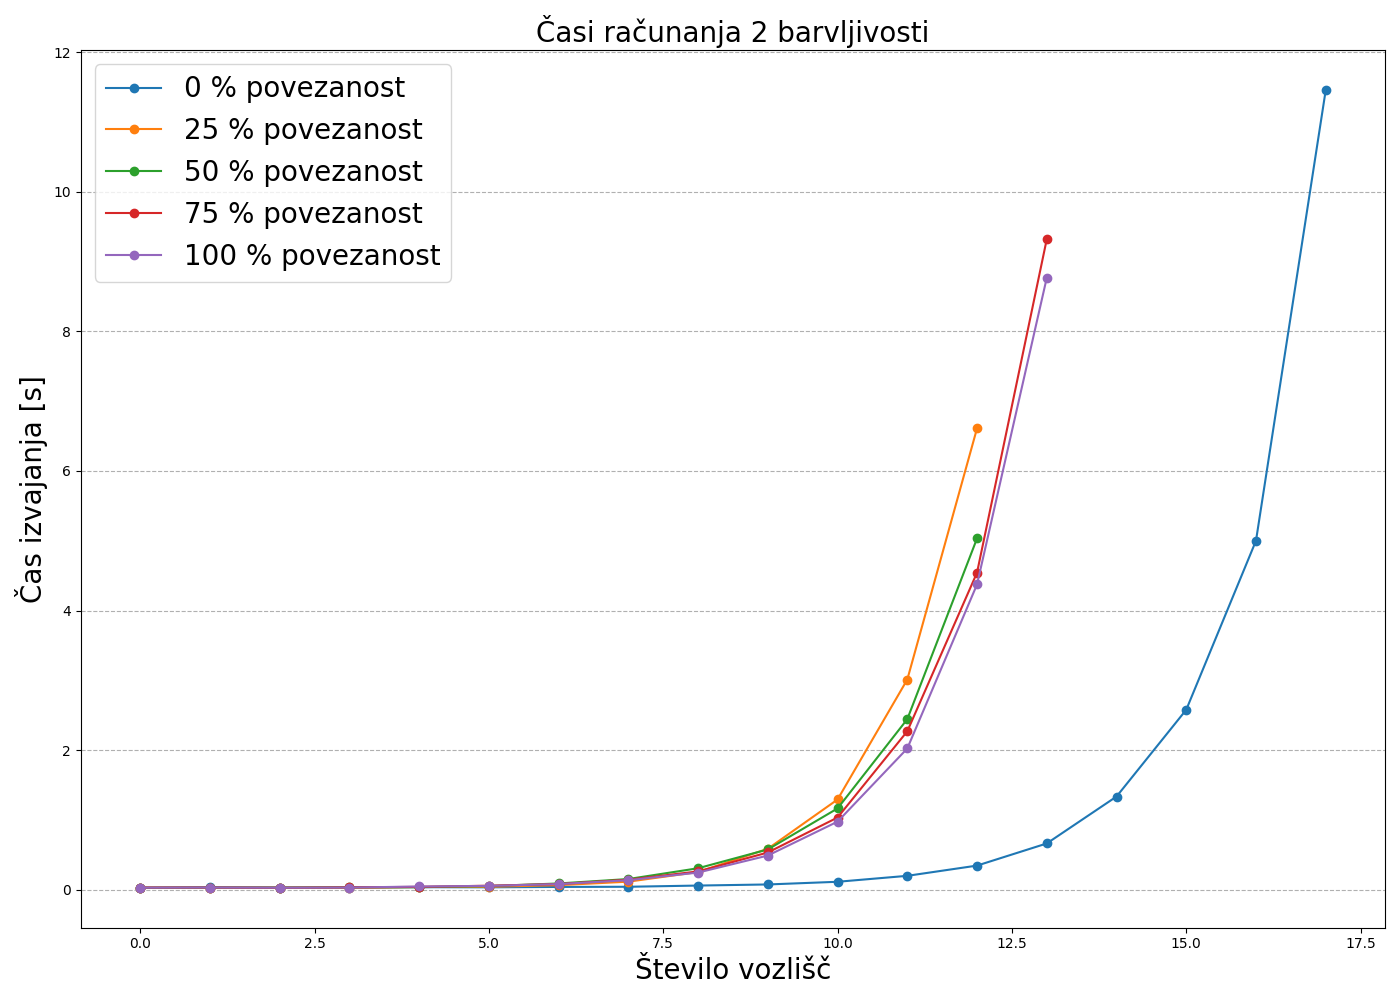
\includegraphics[scale=0.35]{assets/2barvSlow}
\caption{Poraba časa algoritma za preverjanje 2 barvljivosti grafa $G(n, p)$}
\label{slika2}
\end{center}
\end{figure}

\begin{figure}[H]
\begin{center}
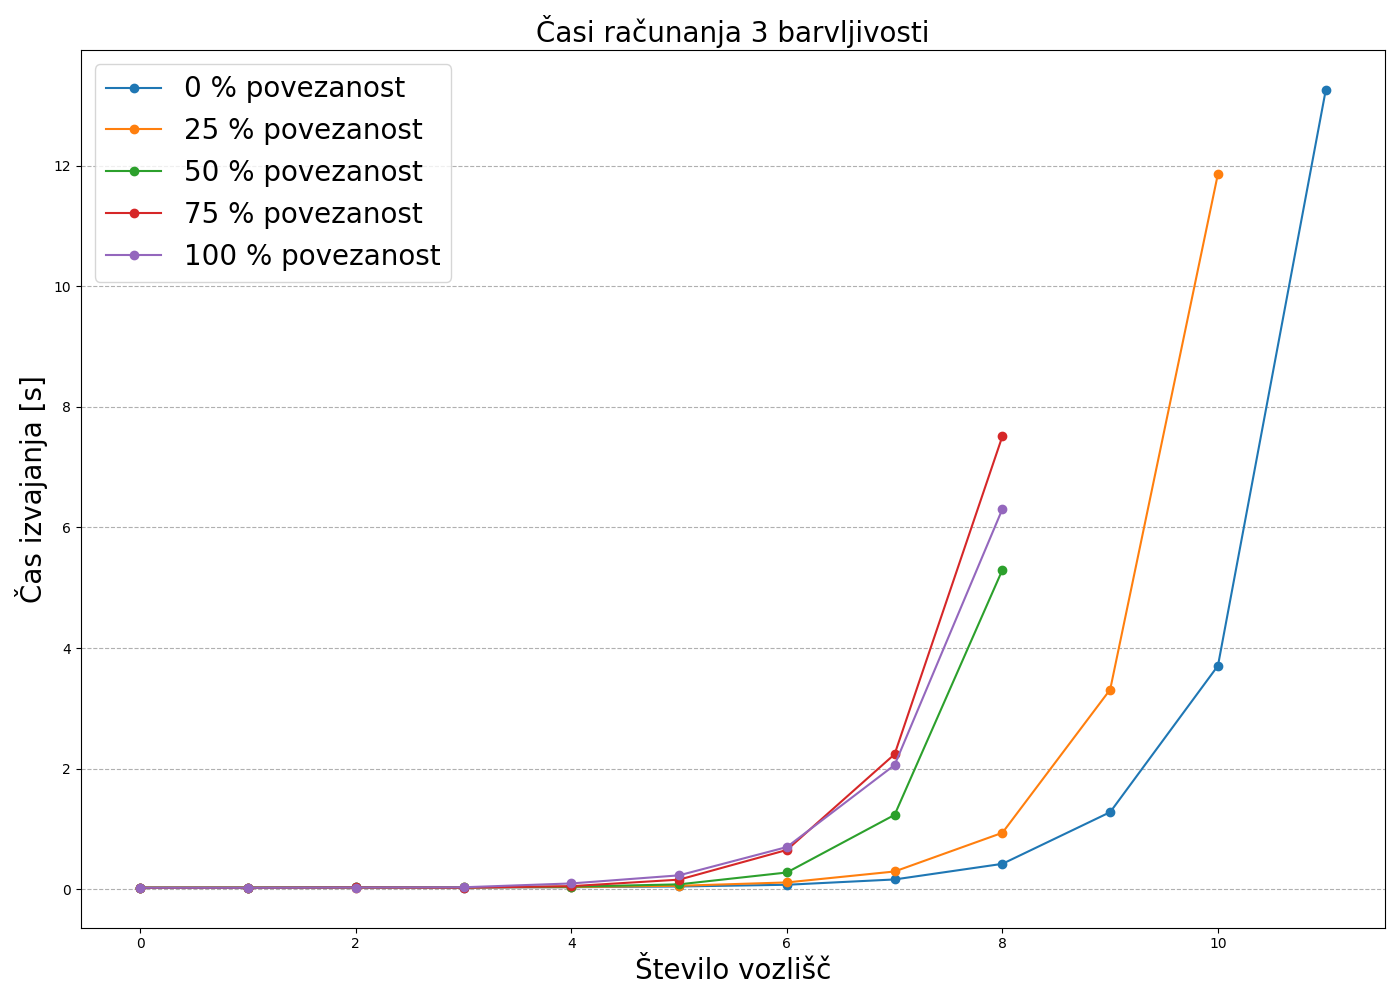
\includegraphics[scale=0.35]{assets/3barvSlow}
\caption{Poraba časa algoritma za preverjanje 3 barvljivosti grafa $G(n, p)$}
\label{slika2}
\end{center}
\end{figure}

\begin{figure}[H]
\begin{center}
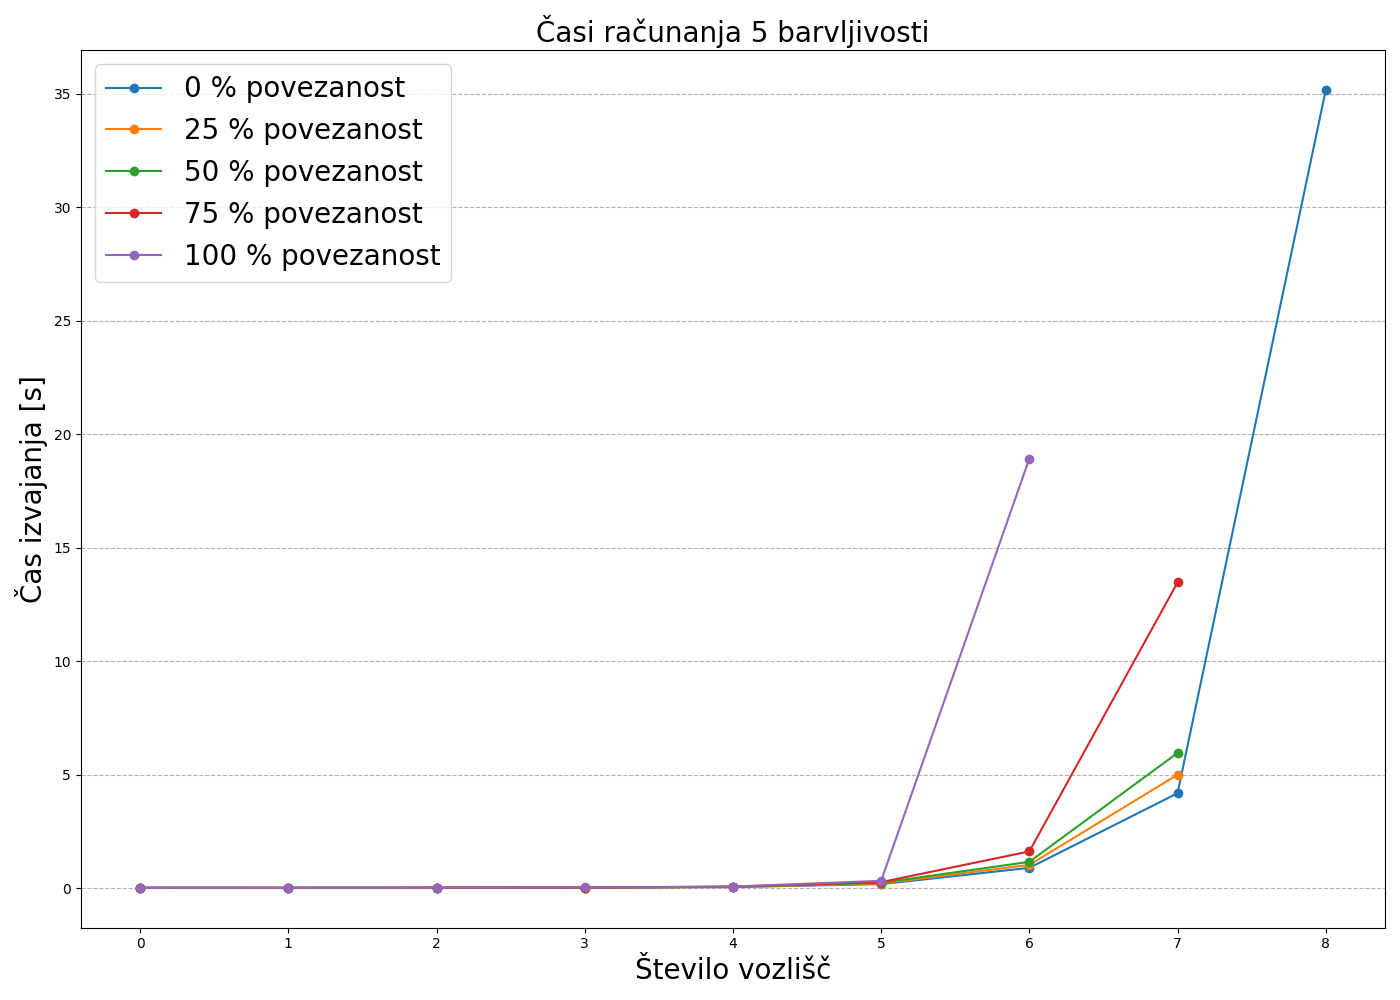
\includegraphics[scale=0.35]{assets/5barvSlow}
\caption{Poraba časa algoritma za preverjanje 5 barvljivosti grafa $G(n, p)$}
\label{slika2}
\end{center}
\end{figure}

Grafe smo pridobili tako, da je Python klical prevejeno Lean kodo in beležil čas izvajanja. Lean program je zgeneriral 1000
naključnih grafov $G(n, p)$ ter za vsakega preveril ali je $k$ barvljiv, kjer je bil $k$ podan kot argument programa.
Čas računanja torej opiše čas porabljen za izračun na 1000 grafih za bolj stabilne rezultate. Program se je izvajal
na računalniku z AMD Ryzen 9 7950x procesorjem in zadostno količino delavnega pomnilnika, kjer pa se nismo posebej trudili
s tem da bi uporabljali več jeder. 

Vidimo da je poraba časa eksponentna v številu vozlišč grafa ter da je preverjanje $k$ barvljivosti za večje $k$ 
počasnejše. To je pričakovano, saj je število možnih barvanj eksponentno v številu vozlišč grafa.
Opazimo, da je pri grafih brez povezav algoritem najhitrejši, vendar še vedno eksponenten. Domnevamo da je to zaradi tega, 
ker Lean najprej generira vsa možna barvanja in šele nato preveri ali je katero veljavno. 

Vidimo da je za preverjanje $3$ in $5$ barvljivosti algoritem počasnejši več kot je povezav, kar je smiselno ker je pri velikem 
številu povezav verjetnost da barvanje obstaja manjše, zato program ne more ustaviti izvajanja ko najde veljavno barvanje. Pri $2$
barvljivosti ta opazka o hitrosti iz neznanih razlogov ne velja. 

Na podoben način smo preizkusili tudi hitrejši algoritem za preverjanje $2$ barvljivosti.
\begin{figure}[H]
\begin{center}
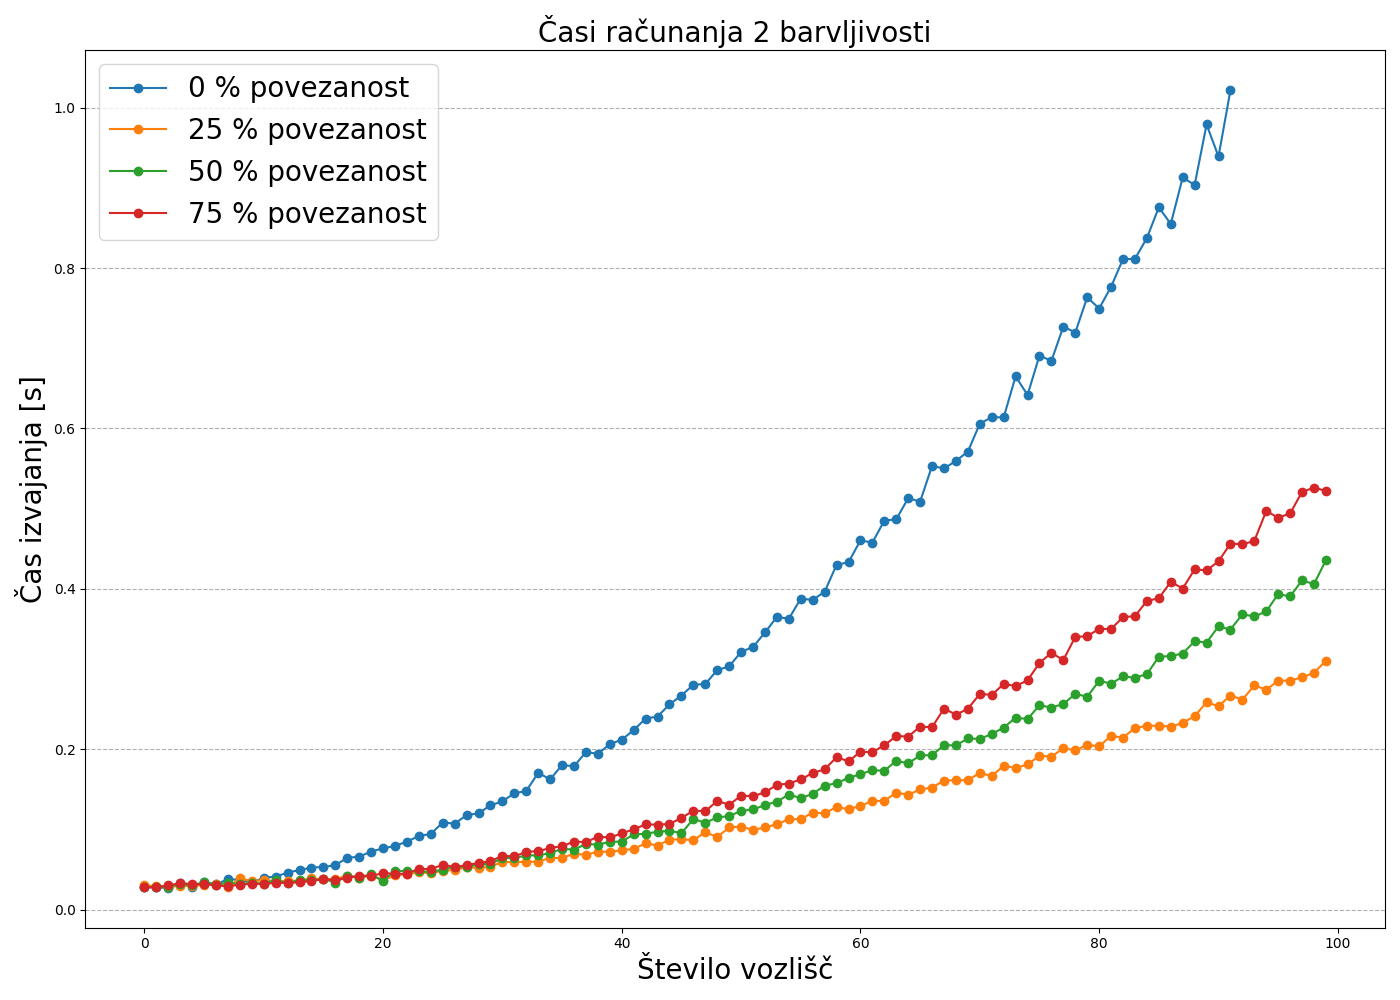
\includegraphics[scale=0.4]{assets/2barvFast}
\caption{Poraba časa hitrega algoritma za preverjanje 2 barvljivosti grafa $G(n, p)$}
\label{slika2}
\end{center}
\end{figure}

Vidimo da je algoritem za katerega smo trdili da je hitrejši brez dokaza (in dokazali pravilnost) res bistveno hitrejši.
Še vedno ima nelinearno časovno zahtevnost, kar pa je smiselno ker imamo recimo $O(n^2)$ povezav z našim $G(n, p)$ modelom.

\section{Zaključek}
Ugotovili smo da je Lean 4 primeren jezik za implementacijo in dokazovanje pravilnosti algoritmov za računanje kromatičnega
števila grafov. Dodane stvari ki bi bile zanimive za raziskovanje so dokazovanje da hiter algoritem vedno deluje pravilno
(torej da vrne pravilno barvanje ali lih cikel in da se ne more zgoditi da mora Lean uporabiti počasno verzijo algoritma),
ugotavljanje večjega števila invariant na grafih ter implementacija hitrih algoritmov s pričami v hitrejših jezikih.
\end{document}
